\documentclass[11pt,a4paper,headinclude,footinclude,chapterprefix=on]{scrreprt} 
\usepackage[utf8]{inputenc} 
\usepackage[T1]{fontenc} 
\usepackage{tabularx} 
\usepackage{multicol} 
\usepackage{graphicx} 
\usepackage{tikz} 
\usepackage{amssymb} 
\usepackage{textcomp}

% ================================================================
% Variables
% ================================================================
\newcommand{\trnumber}{TKN-14} 
\newcommand{\trdate}{March 2014} 
\newcommand{\trauthor}{Aravinth, Sivalingam Panchadcharam} 
\newcommand{\tremail}{contact@aravinth.info} 
\newcommand{\trtitle}{Variations in Wi-Fi RSSI due to different types of Interferences}

% ================================================================
% Page Style
% ================================================================
\usepackage{geometry} \geometry{a4paper, inner=30mm, outer=25mm, top=40mm, bottom=42mm}

\usepackage[headsepline,plainheadsepline,footsepline,plainfootsepline]{scrpage2} \clearscrheadfoot

\ihead[\Large {\scshape TU Berlin }]{\Large {\scshape TU Berlin }}

\ifoot[{\tiny 
\begin{minipage}
	{4.0cm}Copyright at Technical University Berlin. 
	\newline All Rights reserved. 
\end{minipage}
}]{{\tiny 
\begin{minipage}
	{4.0cm}Copyright at Technical University Berlin. 
	\newline All Rights reserved. 
\end{minipage}
}} \cfoot[\scriptsize \trnumber]{\scriptsize \trnumber} \ofoot[Page 
\pagemark]{Page 
\pagemark}

\pagestyle{scrheadings}

\usepackage{mathptmx} 
\usepackage[scaled=.92]{helvet} 
\usepackage{courier}

\addtokomafont{pagefoot}{\normalfont}

% ================================================================
% ================================================================
\begin{document}

\bibliographystyle{plain}

% ================================================================
% Cover Sheet
% ================================================================
{ \sffamily

\thispagestyle{empty}
\begin{tabularx}
	{\columnwidth}{cXc} 
	
\includegraphics[height=1cm]{TU-Logo-3D-rot.pdf} & & 
	
\includegraphics[height=1cm]{tknlogo.pdf} \\
\end{tabularx}

\vspace{1.0cm}
\begin{center}
	{\huge 
	\noindent Technical University Berlin
	
	\vspace{0.5cm}
	
	\noindent Telecommunication Networks Group
	\begin{center}
		\rule{15.5cm}{0.4pt} 
	\end{center}
	} 
\end{center}
\begin{minipage}
	[][11.0cm][c]{14.5cm} {\Huge
	\begin{center}
		\trtitle 
	\end{center}
	\begin{center}
		\trauthor \\
		{\Large \tremail} 
	\end{center}
	\begin{center}
		Berlin, \trdate 
	\end{center}
	
	\vspace{0.5cm}
	
	}
	
	%\begin{center}
	%\setlength{\fboxrule}{2pt}\setlength{\fboxsep}{2mm}
	%\fbox{TKN Technical Report \trnumber}
	%\end{center}
\end{minipage}

\setlength{\fboxrule}{0.4pt} \setlength{\fboxsep}{0.4pt}
\begin{center}
	
	\rule{15.5cm}{0.4pt}
	
	\vspace{0.5cm}
	
	{\huge {Project in advanced network technologies}}
	
	\vspace{0.5cm}
	
	{\huge Supervisors: Dr. Arash Behboodi, Filip Lemic}
	
	\vspace{0.5cm}
\end{center}
}

% ================================================================
% Abstract
% ================================================================
\begin{abstract}
	\subsection*{\abstractname} WiFi Beacon packets are transmitted periodically to announce the presence of WLAN. RSSI is Received Signal Strength Indicator which indicates the power of signal that is received at the receiver. Beacon Packet RSSI values are extensively used for ranging and localization purpose. However, RSSI value changes with various interferences, different chipsets and distance. This project work includes an implementation of a software tool to visualize the raw data obtained during the experiments and examines how these RSSI values changed by controlled interferences. 
\end{abstract}

% ================================================================
% Tableofcontents
% ================================================================
\tableofcontents

% ================================================================
% Introduction
% ================================================================
{ 
\chapter{Introduction} 
\section*{Beacon Packet} In Wireless Local Area Network (WLAN) Beacon Packets are transmitted periodically to announce the presence of WiFi Network. It contains information of the network such as SSID, BSSID and type of encryption.

\section*{Received Signal Strength Indicator (RSSI)} It indicates the power of signal which is received at the receiver and included into the beacon packet by Network Interface Card. }

% ================================================================
% Problem Statement
% ================================================================
{ 
\chapter{Problem Statement} }

% ================================================================
% RSSI Visualization Tool
% ================================================================
{ 
\chapter{RSSI Visualization Tool} }

% ================================================================
% Design
% ================================================================
\chapter{Design} 
\section{Interference} 
\subsection{Introduction} This document shortly presents initial interference scenarios that will be artificially generated in TKN Wireless Indoor Sensor network Testbed (TWIST) testbed in order to benchmark different indoor localization solutions in the environments with controlled interference. The reason for benchmark representative indoor localization solutions in the environments with con- trolled interference is to determine if and to which extend different types and amounts of Radio Frequency (RF) interference can influence the indoor localization performance. 
\subsection{Interference Scenarios}

\subsubsection{Reference Scenario} 
\begin{figure}
	[h] \centering 
	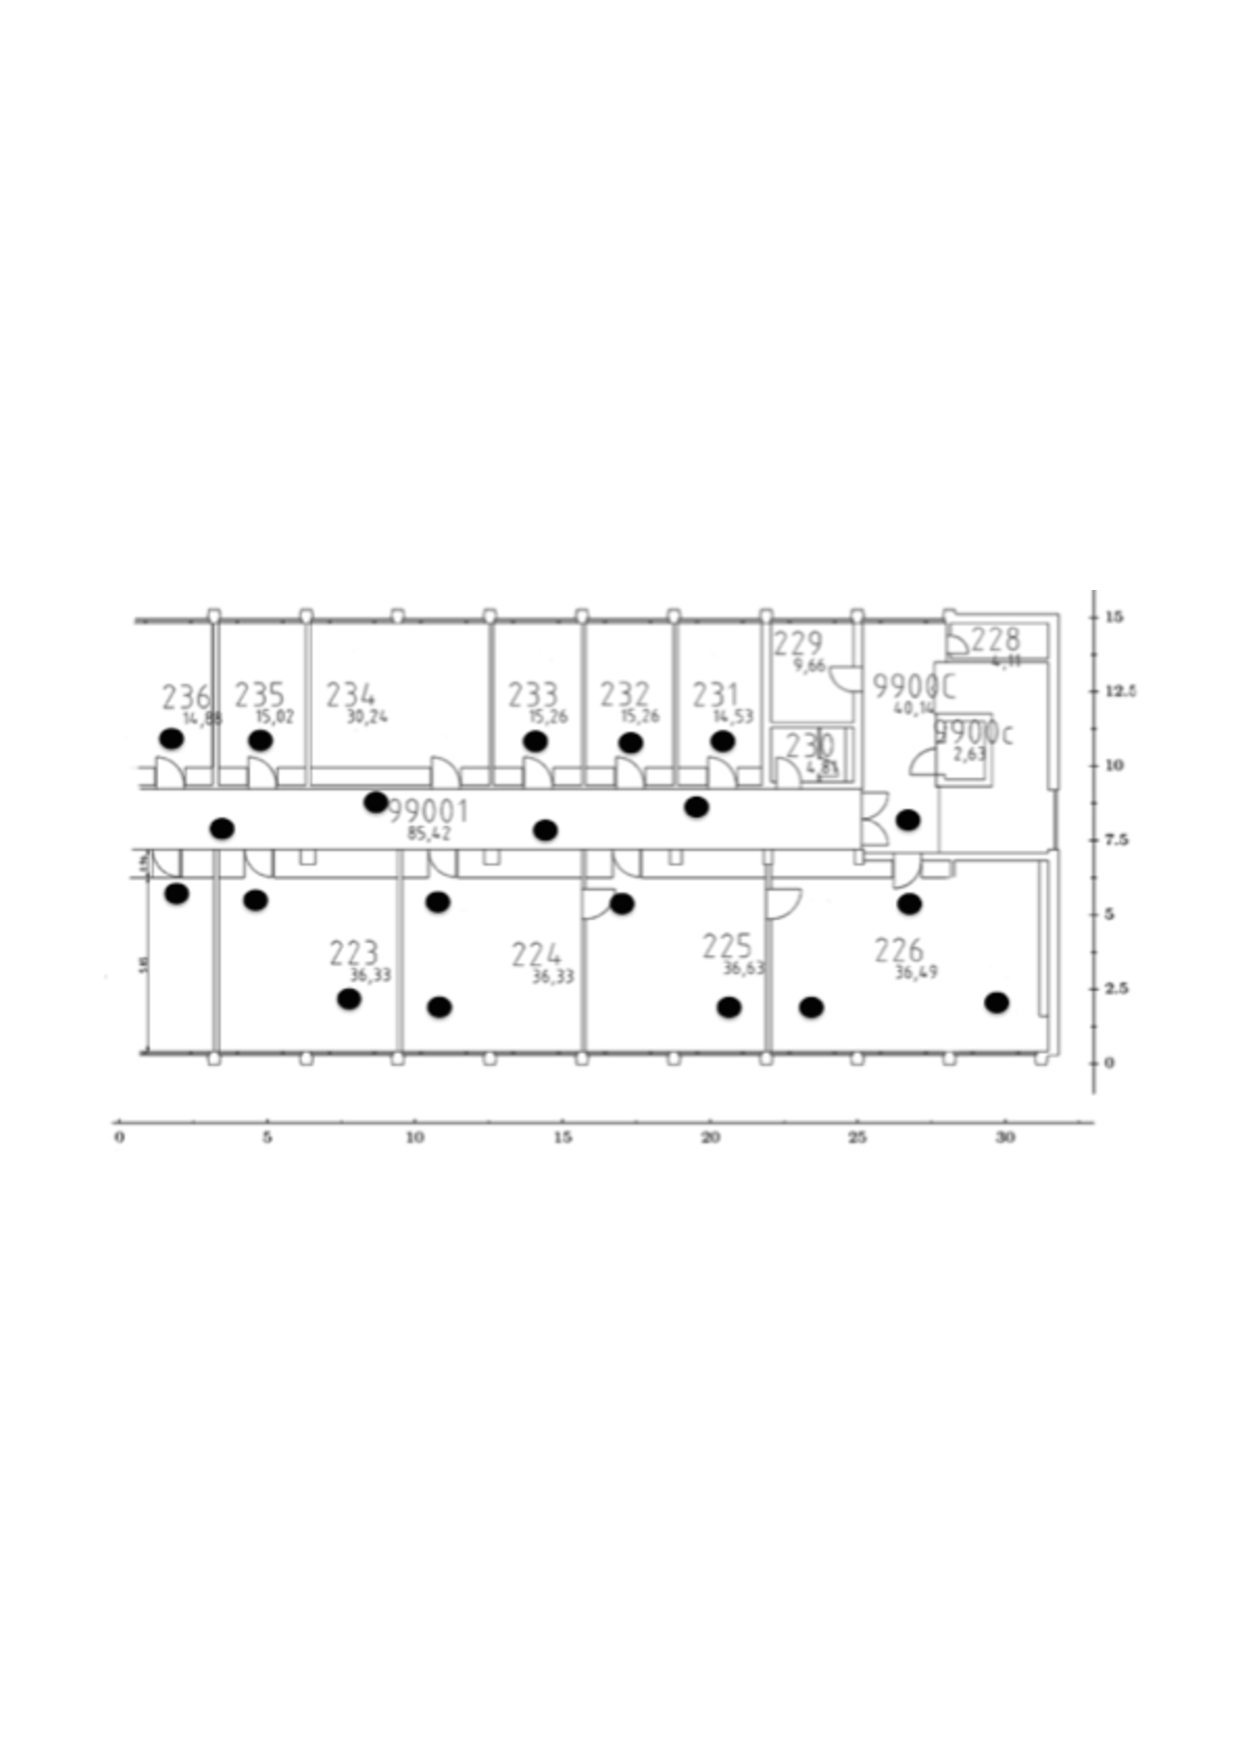
\includegraphics[width=100mm]{floor} \caption{Locations of measurement points} \label{fig:logo} 
\end{figure}

This reference scenario is instantiated on the 2nd floor of the TWIST testbed in Berlin. It is called “Reference scenario”, while no artificial interference is generated and the presence of uncontrolled interference is minimized. Ac- cording to the EVARILOS Benchmarking Handbook (EBH), this scenario is an instance of the “Small office” type of scenarios. In this scenario 20 measurement points are defined and their locations are given in Figure 1.

\paragraph{} At each measurement point the indoor localization System Under Test (SUT) is requested to estimate location. The SUT device is carried to each measurement location using the robotic platform. The navigation stack of the robotic platform gives one order of magnitude more accurate location estimation than considered SUTs and the location obtained from the robotic platform is considered as the ground truth.

\paragraph{} The experiments were performed at the weekend afternoon, so the influence of interferes has been minimized. Furthermore, the wireless spectrum has been measured using the WiSpy device attached to the robotic platform and all measurements with the interference threshold above certain level have been repeated. Finally, before each experiment a more detained measurement of the spectrum has been taken with the spectrum analyzer at a predefined location.

\subsubsection{Interference Scenario 1} First interference scenario instantiated in TWIST testbed uses the testbed Wireless Fidelity (WiFi) nodes as interference sources. Interference type is jamming on one IEEE 802.11 channel with the maximum transmission power. Three of such jamming nodes are present at different locations in the testbed environment. Summary of this interference scenario is given in Table 1.

\begin{table}
	[h] \centering \caption{Interference scenario summary} \label{tb:table} 
	\begin{tabular}
		{|l|l|} \hline \multicolumn{2}{|c|}{Types of interference sources} \\
		\hline WiFi & \checkmark \\
		Microwave & \texttimes \\
		DECT & \texttimes \\
		Bluetooth & \texttimes \\
		3G & \texttimes \\
		ZigBee & \texttimes \\
		\hline \multicolumn{2}{|c|}{Types of interference sources} \\
		\hline Number of sources & 3 \\
		Power & 20 dBm \\
		Waveform & Carrier jamming \\
		Specific pattern & \\
		Start \& stop time & Beginning \& end of experiment \\
		Traffic model & \\
		\hline \multicolumn{2}{|c|}{Traffic parameters of interference} \\
		\hline Packet size & \\
		Inter-packet gap & \\
		Bit rate & \\
		File size & \\
		Start \& stop size & \\
		Traffic model & \\
		\hline \multicolumn{2}{|c|}{Network parameters} \\
		\hline Network size & \\
		Node density & \\
		Node mobility & \\
		Node failures & \\
		\hline 
	\end{tabular}
\end{table}

\subsubsection{Interference Scenario 2}In this interference scenario instantiated in TWIST testbed interference is created using the IEEE 802.15.4 Tmote Sky nodes. The interference type is jamming on one IEEE 802.15.4 channel with a constant transmit power equal to 0 dBm. Five of these jamming nodes will be present in the testbed environment. Summary of this interference scenario is given in Table 2.

\begin{table}
	[h] \centering \caption{Interference scenario summary} \label{tb:table} 
	\begin{tabular}
		{|l|l|} \hline \multicolumn{2}{|c|}{Types of interference sources} \\
		\hline WiFi & \texttimes \\
		Microwave & \texttimes \\
		DECT & \texttimes \\
		Bluetooth & \texttimes \\
		3G & \texttimes \\
		ZigBee & \checkmark \\
		\hline \multicolumn{2}{|c|}{Types of interference sources} \\
		\hline Number of sources & 5 \\
		Power & 0 dBm \\
		Waveform & Carrier jamming \\
		Specific pattern & \\
		Start \& stop time & Beginning \& end of experiment \\
		Traffic model & IEEE 802.15.4 radio \\
		\hline \multicolumn{2}{|c|}{Traffic parameters of interference} \\
		\hline Packet size & \\
		Inter-packet gap & \\
		Bit rate & \\
		File size & \\
		Start \& stop size & \\
		Traffic model & \\
		\hline \multicolumn{2}{|c|}{Network parameters} \\
		\hline Network size & \\
		Node density & \\
		Node mobility & \\
		Node failures & \\
		\hline 
	\end{tabular}
\end{table}

\subsubsection{Interference Scenario 3}Second interference scenario instantiated in TWIST testbed defines interference types that is usual for the office and home environments. Namely, interference is emulated using 4 WiFi embedded Personal Computers (PCs), namely a server, email client, data client, and video client. The server acts as a WiFi Access Point (AP) and a gateway for the emulated services. The email client will “check email” once every 15 seconds for a duration of one second. The data client is emulated via TCP streams one starting at 45 seconds for a duration of 22.5 seconds and the other starting at 105 seconds for a duration of 45 seconds. The video client is emulated as a UDP stream of 100 kbps for half the experiment cycle and it will start at the middle of the experiment. In total, the experiment takes 150 seconds. Summary of this interference scenario is given in Table 3.

\begin{table}
	[h] \centering \caption{Interference scenario summary} \label{tb:table} 
	\begin{tabular}
		{|l|l|} \hline \multicolumn{2}{|c|}{Types of interference sources} \\
		\hline WiFi & \checkmark \\
		Microwave & \texttimes \\
		DECT & \texttimes \\
		Bluetooth & \texttimes \\
		3G & \texttimes \\
		ZigBee & \texttimes \\
		\hline \multicolumn{2}{|c|}{Types of interference sources} \\
		\hline Number of sources & 3 \\
		Power & 20 dBm \\
		Waveform & \\
		Specific pattern & \\
		Start \& stop time & Beginning \& end of experiment \\
		Traffic model & WiFi traffic \\
		\hline \multicolumn{2}{|c|}{Traffic parameters of interference} \\
		\hline Packet size & \\
		Inter-packet gap & \\
		Bit rate & \\
		File size & \\
		Start \& stop size & \\
		Traffic model & \\
		\hline \multicolumn{2}{|c|}{Network parameters} \\
		\hline Network size & \\
		Node density & \\
		Node mobility & \\
		Node failures & \\
		\hline 
	\end{tabular}
\end{table}

% ================================================================
% Experiments
% ================================================================
{ 
\chapter{Experiments} }

% ================================================================
% Re
% ================================================================
{ 
\chapter{Results} }

% ================================================================
% Conclusion
% ================================================================
{ 
\chapter{Conclusion} }

\pagebreak
\begin{thebibliography}
	{9} \bibitem{lamport94} Leslie Lamport \bibitem{lamport95} Leslie Lamport 
\end{thebibliography}

\end{document}
